\documentclass[10pt]{article}

% Manage page layout
\usepackage[margin=2.5cm, includefoot, footskip=30pt]{geometry}
\pagestyle{plain}
\setlength{\parindent}{0em}
\setlength{\parskip}{1em}
\renewcommand{\baselinestretch}{1}

%%%%%%%PACKAGES HERE%%%%%%%
\usepackage{tikz}
\usepackage{amsmath}
\usepackage{amssymb}
\usepackage{graphicx}
\usepackage{subcaption}
\usepackage{standalone}

\newcommand{\R}{\mathbb{R}}
\newtheorem{theorem}{Theorem}
\newtheorem{lemma}[theorem]{Lemma}
\usetikzlibrary{decorations.pathmorphing, decorations.pathreplacing, angles,
                quotes, calc, er, positioning}
%%%%%%%%%%%%%%%%%%%%%%%%%%%
\title{Memory size in the Prisoner's Dilemma}
\author{Nikoleta E. Glynatsi \and Vincent Knight}
\date{}

\begin{document}

\maketitle

\begin{abstract}

The two player Iterated Prisoner's Dilemma is a fundamental iterated game used
for studying the emergence of cooperation. The two players interact repeatedly
and they have the ability to adopt strategies. A strategy allows a player to map
the outcomes of the previous interactions to an action. A set of strategies that
consider only the outcome of the previous round are called memory one. These
players gain attention after a publication in 2012 that showed that a memory one
strategy can manipulate its opponent.

In this manuscript we build upon a framework provided in 1989 for the study of
these strategies and identify the best responses of memory one players. The aim
of this work is to show the limitations of memory one strategies in multi-opponent
interactions. A number of theoretic results are presented.
%TODO: Expand when we get results
\end{abstract}

\section{Introduction}\label{section:introduction}

The Prisoner's Dilemma (PD) is a two player person game used in understanding the
evolution of co-operative behaviour. Each player can choose between cooperation
(C) or defection (D). The decisions are made simultaneously and independently.
The normal form representation of the game is given by:

\begin{equation}\label{equ:pd_definition}
    S_p = \begin{pmatrix}
    R & S  \\
    T & P
    \end{pmatrix} \quad
    S_q = \begin{pmatrix}
        R & T  \\
        S & P
        \end{pmatrix}
\end{equation}

where \(S_p\) represents the utilities of the first player and \(S_q\) the utilities
of the second player. The payoffs, \((R, P, S, T)\), are constrained by equations
(\ref{eq:pd_constrain_one}) and~(\ref{eq:pd_constrain_two}). Constrain
(\ref{eq:pd_constrain_one}) ensures that defection dominates cooperation and
constrain (\ref{eq:pd_constrain_two}) ensures that there is a dilemma. Because
the sum of the utilities for both players is better when both choose cooperation.
The most common values used in the literature are \((3, 1, 0, 5)\)~\cite{Axelrod1981}.

\begin{equation}\label{eq:pd_constrain_one}
    T > R > P > S 
\end{equation}

\begin{equation}\label{eq:pd_constrain_two}
    2R > T + S
\end{equation}

The PD is a one shot game, however it is commonly studied in a manner where the
history of the interactions matters. The repeated form of the game is called the
Iterated Prisoner's Dilemma (IPD) and in the 1980s following the work of
\cite{Axelrod1980a, Axelrod1980b} it attracted the attention of the scientific
community.

In~\cite{Axelrod1980a} a computer tournament of the IPD was performed. A
tournament is a series of rounds of the IPD between pairs of strategies. The
topology commonly used, \cite{Axelrod1980a, Axelrod1980b}, is that of a round
robin where all contestants compete against each other. The winner of these
tournament was decided on the average score and not in the number of wins.

These tournaments were the milestones of an era which to today is using
computer tournaments to explore the robustness of strategies of IPD. Though
the robustness can also be checked through evolutionary process~\cite{Nowak}.
However, this aspect will not be considered here, instead the focus is on
performance in tournaments.

In Axelrod's original tournaments \cite{Axelrod1980a, Axelrod1980b}, strategies
were allowed access to the history and in the first tournament they also knew
the number of total turns in each interaction. The history included the
previous moves of both the player and the opponent. How many turns of history
that a strategy would ue, the memory size, was left to the creator of the
strategy to decide. For example the winning strategy of the first tournaments,
Tit for Tat was a strategy that made use of the previous move of the opponent
only. Tit for Tat is a strategy that starts by cooperating and then mimics the
previous action of it's opponent. Strategies like Tit for Tat are called memory
one strategies. A framework for studying memory one strategies was introduced
in~\cite{Nowak1989} and further used in~\cite{Nowak1993, Nowak1990}.

In~\cite{Press2012} Press and Dyson, introduced a new set of memory one
strategies called zero determinant (ZD) strategies. The ZD strategies,
manage to force a linear relationship between the score of the strategy
and the opponent. Press and Dyson, prove their concept of the ZD strategies
and claim that a ZD strategy can outperform any given opponent.

The ZD strategies have tracked a lot of attention. It was stated that
``Press and Dyson have fundamentally changed the viewpoint on the Prisoner's
Dilemma''~\cite{Stewart2012}. In~\cite{Stewart2012}, the Axelrod's
tournament have been re-run including ZD strategies and a new set of ZD
strategies the Generous ZD. Even so, ZD and memory one strategies have
also received criticism. In~\cite{Harper2015}, the `memory of a strategy does
not matter' statement was questioned. A set of more complex strategies,
strategies that take in account the entire history set of the game, were
trained and proven to be more robust than ZD strategies.

\section{Problem Description}

The work of~\cite{Press2012} is considered a milestone in the study of the IPD.
The authors managed to discover a new family of memory on strategies that are
able to manipulate another player. Their work however suffered from limitations.
Only pair wise interactions are taken into account and not multi agent interactions;
interactions in a tournament setting.

This manuscript will consider an optimisation approach to identify the best
response memory one strategy. That will be done for a given opponent as well as
in tournaments. The aim of this work in to:

\begin{itemize}
    \item construct compact methods of identifying best responses.
    \item numerically tests the analytical methods.
    \item prove that memory one strategies suffer for their memory size constrain.
\end{itemize}

The search of best responses will be considered as an optimisation problem.
In the following section the formulation is introduced as well as the objective
function.

\subsection{Utility}

The objective function in a match of the IPD can be no other than the utility
the players receive at the end of the match. More specifically we will consider
the utility of a given memory one strategy against another such strategy.

Initially we properly define memory one strategies. A memory one strategy \(p\)
in a match against a strategy \(q\) would decide it's next action in turn based
on only what occurred in the previous turn. If a strategy is concerned with only
the outcome of a single turn then there are four possible `states' the strategy
could be in. These are \(CC, CD, DC,CC\). A memory one strategy is denoted by the
probabilities of cooperating after each of these states,
\(p=p_1, p_2, p_3, p_4 \in \R_{[0,1]} ^ 4\) as shown by Figure~\ref{fig:diagrammatic_mem_one}.

\begin{figure}
    \begin{center}
    \begin{subfigure}{0.45\textwidth}
        \includestandalone[width=.6\textwidth]{tex/states}
        \caption{Diagrammatic representation of a memory one strategy.}
        \label{fig:diagrammatic_mem_one}
    \end{subfigure}
    \begin{subfigure}{0.45\textwidth}
        \includestandalone[width=.85\textwidth]{tex/markov_chain}
        \caption{Markov chain.}
        \label{fig:markov_chain}
    \end{subfigure}
    \end{center}
\end{figure}

In~\cite{Nowak1990} a framework was introduced by to study the interactions of memory
strategies as a stochastic process. It was described how a match between players
\(p\) and \(q\) can be modelled as a stochastic process, where the players move
from state to  state. More specifically, it can be modelled by the use of a Markov
process of four states, shown in Figure~\ref{fig:markov_chain}.

The transition probability matrix is defined as \(M\) and is given
by,

\begin{equation}\label{eq:m_matrix}
    M = \left[\begin{matrix}p_{1} q_{1} & p_{1} \left(- q_{1} + 1\right) & q_{1} \left(- p_{1} + 1\right) & \left(- p_{1} + 1\right) \left(- q_{1} + 1\right)\\p_{2} q_{3} & p_{2} \left(- q_{3} + 1\right) & q_{3} \left(- p_{2} + 1\right) & \left(- p_{2} + 1\right) \left(- q_{3} + 1\right)\\p_{3} q_{2} & p_{3} \left(- q_{2} + 1\right) & q_{2} \left(- p_{3} + 1\right) & \left(- p_{3} + 1\right) \left(- q_{2} + 1\right)\\p_{4} q_{4} & p_{4} \left(- q_{4} + 1\right) & q_{4} \left(- p_{4} + 1\right) & \left(- p_{4} + 1\right) \left(- q_{4} + 1\right)\end{matrix}\right].
\end{equation}

Let \(v\) be the vector of the stationary probabilities of \(M\) and \(S_p\)
payoff vector of player \(p\). The states of vector \(v\) are given in the
Appendix. The scores of each player can be
retrieved by multiplying the probabilities of each state, at the stationary state,
with the equivalent payoff. Thus, the  utility for player \(p\) against \(q\),
denoted as \(u_q(p)\), is defined by,

\begin{equation}\label{eq:press_dyson_utility}
    u_q(p) = v \times S_p.
\end{equation}

\begin{theorem}\label{theorem:quadratic_form_u}
    For a given memory one strategy \(p\in\mathbb{R}_{[0,1]}^4\) playing another 
    memory one strategy \(q\in\mathbb{R}_{[0,1]}^4\), the 
    utility of the player \(u_q(p)\) can be re written as a ratio of two quadratic
    forms:
    
    \begin{equation}\label{eq:optimisation_quadratic}
    u_q(p) = \frac{\frac{1}{2}p^TQp + c^Tp + a}
                {\frac{1}{2}p^T\bar{Q}p + \bar{c}^Tp + \bar{a}}, 
    \end{equation}
    where \(Q, \bar{Q}\) are matrices of \(4 \times 4\) defined with the transition
    probabilities of the opponent's transition probabilities \(q_1, q_2, q_3, q_4\).
    
    \begin{center}
    \begin{equation}
    \resizebox{0.9\linewidth}{!}{\arraycolsep=2.5pt%
    \boldmath\(
    Q = \left[\begin{matrix}0 & 5 q_{4} \left(q_{1} - q_{3}\right) & - q_{4} \left(q_{1} - q_{2}\right) & \left(q_{1} - q_{4}\right) \left(q_{2} - 5 q_{3} - 1\right)\\5 q_{4} \left(q_{1} - q_{3}\right) & 0 & - 3 q_{4} \left(q_{2} - q_{3}\right) & \left(q_{3} - q_{4}\right) \left(5 q_{1} - 3 q_{2} - 2\right)\\- q_{4} \left(q_{1} - q_{2}\right) & - 3 q_{4} \left(q_{2} - q_{3}\right) & 0 & - \left(q_{2} - q_{4}\right) \left(q_{1} - 3 q_{3} - 1\right)\\\left(q_{1} - q_{4}\right) \left(q_{2} - 5 q_{3} - 1\right) & \left(q_{3} - q_{4}\right) \left(5 q_{1} - 3 q_{2} - 2\right) & - \left(q_{2} - q_{4}\right) \left(q_{1} - 3 q_{3} - 1\right) & 0\end{matrix}\right]\)},
    \end{equation}
    \begin{equation}\label{eq:q_bar_matrix}
    \resizebox{0.8\linewidth}{!}{\arraycolsep=2.5pt%
    \boldmath\(
    \bar{Q} =  \left[\begin{matrix}0 & - \left(q_{1} - q_{3}\right) \left(q_{2} - q_{4} - 1\right) & \left(q_{1} - q_{2}\right) \left(q_{3} - q_{4}\right) & \left(q_{1} - q_{4}\right) \left(q_{2} - q_{3} - 1\right)\\- \left(q_{1} - q_{3}\right) \left(q_{2} - q_{4} - 1\right) & 0 & \left(q_{2} - q_{3}\right) \left(q_{1} - q_{4} - 1\right) & \left(q_{1} - q_{2}\right) \left(q_{3} - q_{4}\right)\\\left(q_{1} - q_{2}\right) \left(q_{3} - q_{4}\right) & \left(q_{2} - q_{3}\right) \left(q_{1} - q_{4} - 1\right) & 0 & - \left(q_{2} - q_{4}\right) \left(q_{1} - q_{3} - 1\right)\\\left(q_{1} - q_{4}\right) \left(q_{2} - q_{3} - 1\right) & \left(q_{1} - q_{2}\right) \left(q_{3} - q_{4}\right) & - \left(q_{2} - q_{4}\right) \left(q_{1} - q_{3} - 1\right) & 0\end{matrix}\right]\)}.
    \end{equation}
    \end{center}
    
    \(c \text{ and } \bar{c}\), are \(4 \times 1\) vectors defined by the transition rates 
    \(q_1, q_2, q_3, q_4\).
    
    \begin{equation}\label{eq:q_matrix_numerator}
    \resizebox{0.3\linewidth}{!}{\arraycolsep=2.5pt%
    \(c = \left[\begin{matrix}- 5 q_{1} q_{4}\\5 q_{4} \left(q_{3} - 1\right)\\q_{4} \left(2 q_{2} + 1\right)\\5 q_{1} q_{4} - 2 q_{2} q_{4} - q_{2} - 5 q_{3} q_{4} + 5 q_{3} - 3 q_{4} + 1\end{matrix}\right]\),}
    \end{equation}
    \begin{equation}\label{eq:q_matrix_denominator}
    \resizebox{0.3\linewidth}{!}{\arraycolsep=2.5pt%
    \(\bar{c} = \left[\begin{matrix}q_{1} \left(q_{2} - q_{4} - 1\right)\\- \left(q_{3} - 1\right) \left(q_{2} - q_{4} - 1\right)\\- q_{1} q_{2} + q_{2} q_{3} + q_{2} - q_{3} + q_{4}\\q_{1} q_{4} - q_{2} - q_{3} q_{4} + q_{3} - q_{4} + 1\end{matrix}\right]\).
    }
    \end{equation}
    
    Lastly, \(a = 5 q_{4}\) and 
    \(\bar{a} = - q_{2} + q_{4} + 1\).
    \end{theorem}

\subsubsection{Validation}

All results are validated using~\cite{axelrodproject} which is an open research
framework for the study of the Iterated Prisoner's Dilemma. This package is
described in~\cite{Knight2016}.

To validate the formulation of \(u_q(p)\) several memory one players were 
matched against 20 opponents. Note that the payoff values  used hereafter in this
work are \((3, 1, 0, 5)\). 
The simulated value of \(u_q(p)\) has been calculated using \cite{axelrodproject}
and the theoretical by  substituting in equation~(\ref{eq:optimisation_quadratic}).
In Figure~\ref{fig:analytical_simulated}, both the simulated and the theoretical
value of \(u_q(p)\), against each opponent, are plotted for three different memory
one strategies. Figure \ref{fig:analytical_simulated} indicates that the 
formulation of \(u_q(p)\) as a quadratic ratio successfully captures the 
simulated behaviour.

\begin{figure}[!htbp]
\begin{center}
    \begin{subfigure}{0.45\textwidth}
        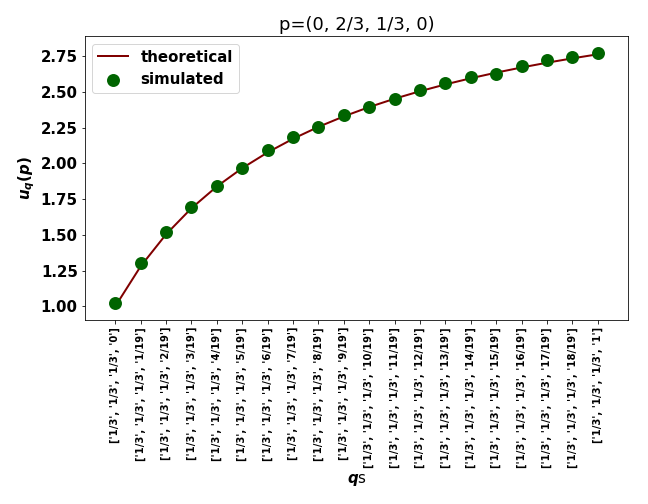
\includegraphics[width=\linewidth]{img/validation_img_two.png}
    \end{subfigure}
    \begin{subfigure}{0.45\textwidth}
        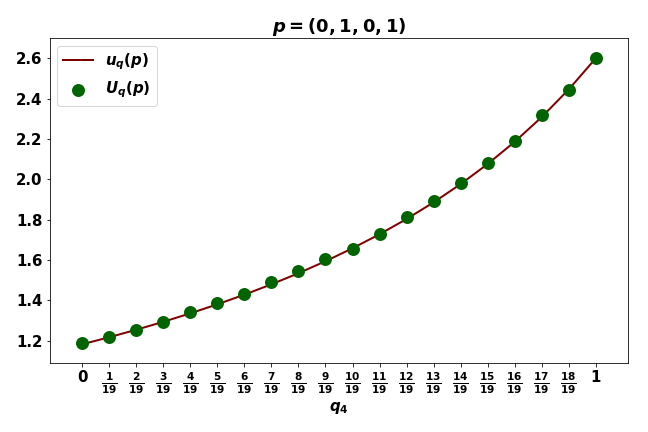
\includegraphics[width=\linewidth]{img/validation_img_three.png}
    \end{subfigure}
\end{center}
\caption{Differences between simulated and analytical results.}
\label{fig:analytical_simulated}
\end{figure}

\section{Best responses Analytically}

The analytical formulation gives the advantage of time. That is because the
payoffs of a match between two opponents are now retrievable without
simulating the actual match itself. Utility \(u_q(p)\) can
now be calculated numerically instead of using simulation. In the introduction
a question was raised: which memory one strategy is the \textbf{best response}
against another memory one?

This will be considered as an optimisation problem, where a memory one strategy
\(p\) wants to optimise it's utility \(u_q(p)\) against an opponent \(q\).
The decision variable is the vector \(p\) and the solitary constrains
\(p \in \R^4_{[0, 1]} \). The optimisation problem is given by~(\ref{eq:mo_optimisation}).

\begin{equation}\label{eq:mo_optimisation}
\begin{aligned}
& \max_p: && \frac{\frac{1}{2}  p  Q  p^T + c^T p + a} 
                  {\frac{1}{2}  p  \bar{Q}  p^T + \bar{c}^T  p + \bar{a}}
\\
& \text{such that}: && \ p \in \R^4_{[0, 1]}.
\end{aligned}
\end{equation}

\subsection{In purely random strategies}

In this section we explore a simplified version of the main problem. A set of
memory one strategies where the transition probabilities of each state are the
same, are called \textbf{purely random strategies}.
as

The optimisation problem of (\ref{eq:mo_optimisation}) now has an extra constraint
and is re written as,

\begin{equation}\label{eq:random_optimisation}
    \begin{aligned}
    \max_p: & \ u_q(p)
    \\
    \text{such that}: & \ p_1 = p_2 = p_3 = p_4 = p \\
        & \ 0 \leq p \leq 1. 
    \end{aligned}
\end{equation}

Note that now \(u_q(p)\) is given by,

\begin{equation}\label{eq:random_utility}
    \begin{aligned}
    u_q(p) & = \frac{n_2p^2 + n_1p +n_0 } {d_1p + d_0}, \ \text{where} \\
    n_2 =  - q_{1} + q_{2} + 2 q_{3} - 2 q_{4},\ n_1 & =  q_{1} - 2 q_{2} - 5 q_{3} + 7 q_{4} + 1, \ n_0 =  q_{2} - 5 q_{4} - 1 \ \text{and}\\
    d_1 =  q_{1} - q_{2} - q_{3} + q_{4},\ d_0 & =  q_{2} - q_{4} - 1. \\
    \end{aligned}
\end{equation}

The utility now is a function of a single variable. Moreover due the format of the
utility we know that the maximum degree is that of a degree equal to 2. Thus
for identifying the best response the following theorem is stated:

\begin{theorem}[Optimisation of purely random player in a match]
\label{theorem:random_optimisation_match}

    The optimal behaviour of a \textbf{purely random} player \((p, p, p, p)\)
    against a memory one opponent \(q\) is given by:

    \[p^* = \textnormal{argmax}(u_q(p)), \ p \in S_q,\]

    where the set \(S_q\) is defined as

    \[S_q = \left \{0, p_{\pm}, 1 \left |
        \begin{array}{l} 0 < p_{\pm} < 1, \\ p_{\pm} \neq \frac{-d_0}{d_1}
        \end{array} \right. \right\}\]
\end{theorem}

Moreover, due the form of the utility for the purely random case, a few interesting cases
have been identified. These are:

\begin{itemize}
    \item Constant case. The plater \(p\) becomes indifferent
    \item Linear case. The utility against \(q\) is linear. Thus the best
    response is a pure strategy.
\end{itemize}

For each case the following Lemmas are stated equivalently. Proofs can be
found in the appendix.

\begin{lemma}\label{lemma:constant}
    A given memory one player, \((q_1, q_2, q_3, q_4)\), makes a \textbf{purely
    random} player, \((p, p, p, p)\), indifferent if and only if, 
    \(-q_1 + q_2 + 2q_3 - 2q_4 = 0 \) and 
    \((q_2 - q_4 - 1)(q_1 - 2q_2 - 5q_3 + 7q_4 + 1) -(q_2 - 5q_4 - 1)(q_1 - q_2 - q_3 + q_4) = 0 \).
    \end{lemma}

\begin{lemma}\label{lemma:linear}
    Against a memory one player, \((q_1, q_2, q_3, q_4)\), a \textbf{purely random}
    player would always play a pure strategy if and only if
    \((q_{1}q_{4} - q_{2} q_{3} + q_{3} - q_{4}) (4 q_{1} - 3 q_{2} - 4 q_{3} + 3 
    q_{4} - 1) = 0\).
    \end{lemma}

Now in a tournament the utility is changed and can be written as:

\begin{equation}\label{eq:tournament_utility}
        \frac{1}{N} \sum_{i=1} ^ {N} {u_q}^{(i)} (p) = \frac{1}{N}
        \frac{\sum\limits_{i=1} ^ {N} (n_2^{(i)} p^2 + n_1^{(i)} p + n_0^
        {(i)}) \prod\limits_{\tiny\begin{array}{l} j=1 \\ j \neq i \end{array}} ^ 
        N (d_1 ^ {(j)}p +
        d_0 ^ {(j)})}{\prod\limits_{i=1} ^ N (d_1 ^ {(i)}p +
        d_0 ^ {(i)})}.
\end{equation}

Let us ignore the coefficients of the utility for now and only consider the degree of \(u_{q(i)} (p)\). Note that the degree of 
\(\sum\limits_{i=1} ^ {N}(n_2^{(i)} p^2 + n_1^{(i)} p + n_0^{(i)})\) is \(N\)
.The sum being multiplied by the product of \(\prod\limits_{\tiny\begin{array}
{l} j=1 \\ j \neq i \end{array}} ^ N (d_1 ^ {(j)}p + d_0 ^ {(j)})\) with a 
degree \(N\). Thus the numerator is determined to be a polynomial of degree 
\(N +1\). The denominator is also a polynomial of degree \(N\). Now that
the degree have been established, equation~(\ref{eq:tournament_utility}) can
be simplified to the following ratio of polynomials:

\begin{equation}\label{eq:utility_polynomial}
    \frac{1}{N} \sum_{i=1} ^ {N} {u_q}^{(i)} (p) =
    \frac{1}{N}\left(\frac{\sum\limits_{i=0}^{N+1} h_i p^i} {\sum\limits_{i=0}^{N}
    k_i p^i}\right)
\end{equation}

Following a similar approach to the study of matches, see equation
(\ref{eq:diff_random_utility}), now \(\frac{du_{q(i)}(p)}{dp}\) can be 
calculated. Differentiating equation~(\ref{eq:tournament_utility}) yields to 
the following:

% \begin{equation}\label{eq:utility_polynomial_diff}
%     \begin{aligned}
%         \frac{d}{dp} \frac{1}{N} \sum_{i=1} ^ {N} {u_q}^{(i)} (p) = &
%         \frac{\frac{d}{dp}\left(\sum\limits_{i = 0} ^ {N + 1} h_ip^i\right)
%                \sum\limits_{i = 0} ^ {N} k_ip^i -
%               \frac{d}{dp}\left(\sum\limits_{i = 0} ^ {N} k_ip^i\right)
%                \sum\limits_{i = 0} ^ {N + 1} h_ip^i}
%              {N\left(\sum\limits_{i = 0} ^ {N + 1} k_ip^i\right)^ 2} \\
%         = &
%         \frac{\sum\limits_{i = 0} ^ {N + 1} ih_ip^{i-1}
%                \sum\limits_{i = 0} ^ {N} k_ip^i -
%                \sum\limits_{i = 0} ^ {N} ik_ip^{i-1}
%                \sum\limits_{i = 0} ^ {N + 1} h_ip^i}
%              {N\left(\sum\limits_{i = 0} ^ {N + 1} k_ip^i\right)^ 2}
%     \end{aligned}
% \end{equation}

Similar to identifying \(p^*\) in match, the roots 
of \(\frac{d}{dp} \frac{1}{N} \sum_{i=1} ^ {N} {u_q}^{(i)} (p)\) alongside the 
bounds compose the candidate set 
of solutions. The roots of 
\(\frac{d}{dp} \frac{1}{N} \sum_{i=1} ^ {N} {u_q}^{(i)} (p)\) are the roots 
only of the numerator, as the denominator can not be nullified. Studying 
equation (\ref{eq:utility_polynomial_diff}), the degree of the numerator can 
be verified to be equal to \(2N\). Thus, the size of roots of the numerator
is equal to \(2N\).

The roots on the polynomial in this work will be calculated using a companion 
matrix method~\cite{Niu2003}. This method allows the roots of the polynomial to
be computed by calculating the eigenvalues of the corresponding companion 
matrix.

Corresponding to Theorem~\ref{theorem:random_optimisation_match}, a theorem 
for \(p^*\) in a tournament is given by Theorem
\ref{theorem:random_optimisation_tournament}.

\begin{theorem}[Optimisation of purely random player in a tournament]
\label{theorem:random_optimisation_tournament}
    The optimal behaviour of a \textbf{purely random} player \((p, p, p, p)\)
    in an \(N-\)memory one player tournament, \(\{q_{(1)}, q_{(2)} \dots,q_{(N)} \}
    \) is given by:

    \[p^* = \textnormal{argmax}(\sum_{i=1} ^ {N} {u_q}^{(i)} (p) ), \ p \in S_{q(i)},\]

    where the set \(S_{q}\) is defined as:

    \[S_{q} = \
    U_{\substack{i=1 \\ \lambda_i \neq \frac{do_i}{d1_i}}} ^ {2N}  \lambda_i \cup \{0, 1\},\]

    and \(\lambda_i\) are the eigenvalues of the companion matrix corresponding to the
    numerator of \[\frac{d}{dp} \frac{1}{N} \sum_{i=1} ^ {N} {u_q}^{(i)} (p).\]
\end{theorem}

Note that the size of candidate solutions is \( 1 \leq|S_{q(i)}| \leq 2N + 2\).

\subsection{In memory one strategies}

\begin{itemize}
    \item Optimisation in matches.
    \item + Lagrange
    \item Optimisation in tournaments.
\end{itemize}

\section{Best responses Numerically}

\begin{itemize}
    \item Purely random in matches. Yes our algorithm works
    \item Purely random in tournaments. Yes our algorithm works
    \item Reactive strategies and resultant theory
    \item Differential evolution
\end{itemize}

\section{Limitation of memory}

\begin{itemize}
    \item Purely random in tournaments, compare with complex
    \item Parameter sweep and how gambler do better?
\end{itemize}

\section{Extra: Stability of defection}

\begin{itemize}
    \item Stability of defection against mem one
    \item Stability of defection against reactive
\end{itemize}


% Bibliography
\bibliographystyle{plain}
\bibliography{bibliography.bib}

\end{document}